\documentclass[a4paper]{article}

\pdfmajorversion=1
\pdfminorversion=7
\pdfcompresslevel=9
\pdfobjcompresslevel=2

\usepackage[hidelinks]{hyperref}
\usepackage[margin=60pt]{geometry}
\usepackage[utf8]{inputenc}
\usepackage[english]{babel}
\usepackage{graphicx}

\setlength{\parindent}{0pt}

\hypersetup{
    pdftitle={Model Identification and Data Analysis - Module 1},
    pdfauthor={Riccardo Motta}
}

\newcommand\nbvspace[1][3]{\vspace*{\stretch{#1}}}

\begin{document}

    \begin{titlepage}

        \begin{center}

            \nbvspace[1]

            
\includegraphics[width=0.3\columnwidth]{./images/polimi}

            \nbvspace[2]

            {\huge \textbf{\textsc{Formal Digital Twin of a LEGO® MINDSTROMS™ Production Plant}}} \\
            [3em]
            {\Large Formal Methods for Concurrent and Real-Time Systems} \\
            [1.5em]
            {\Large A.Y. 2022-2023}

            \nbvspace[8]

            \begin{tabular}{lrp{0.04\columnwidth}lrp{0.04\columnwidth}lr}
                \multicolumn{2}{c}{\Large \textbf{Andrea Infantino}} & & \multicolumn{2}{c}{\Large \textbf{Riccardo Motta}} & & \multicolumn{2}{c}{\Large \textbf{Matteo Negro}} \\
                Person ID & ??? & & Person ID & 10658639 & & Person ID & 10642961 \\
                Student ID & ??? & & Student ID & 218685 & & Student ID & ???
            \end{tabular}

            \nbvspace[1]

        \end{center}

    \end{titlepage}

    \tableofcontents{}

    \pagebreak

    \section{Model Description}

    \subsection{The Production Plant}

    \begin{figure}[h]
        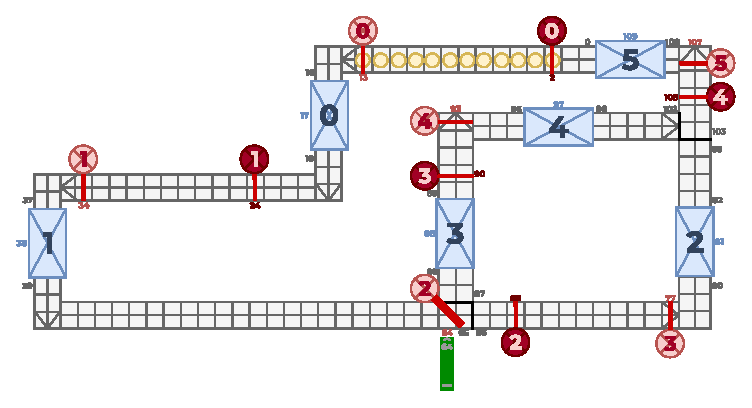
\includegraphics[width=\columnwidth]{./images/plant}
        \caption{the production plant we modelled.}
    \end{figure}

    % TODO: write the differences with the original model (flow controller position and missing slot on top-right corner)

    \subsection{General Overview}

    The model of our system is made of 6 different components which interact between them in order to coordinate the entire production plant. Some of them are also instantiated many times in order to a simpler modelling of the entire system.

    \paragraph{Initializer}

    \paragraph{Conveyor belt}

    \paragraph{Stations}

    \paragraph{Laser sensors}

    \paragraph{Flow controller}

    \subsection{Components Description}

    \section{Scenarios}

    \section{Properties}

    \section{Conclusions}

\end{document}
